%!TEX root=../document.tex

\section{Ergebnisse}
\subsection{Theorie}
\subsection{iSCSI Initiator}
\subsubsection{Basics}
Da openfiler bereits zur Verfügung gestellt wurde, musste keine NAS Appliance installiert und konfiguriert werden.

Die restliche Vorgehensweise entspricht genau der Aufgabenstellung. Zuerst wurde das Ubuntu Package \texttt{open-iscsi} installiert. Nachdem in der Datei \texttt{/etc/iscsi/iscsi.conf} die Authentifizierungsmethode auf CHAP (Challenge Handshake Authentication Protocol) gesetzt und die Anmeldedaten konfiguriert wurden, konnte auch schon die Liste der verfügbaren Targets ausgegeben werden.

\begin{lstlisting}[style=bash, caption=Verfügbare Targets]
daniel@daniubuntu:~$ sudo iscsiadm -m discovery -t sendtargets -p 10.0.106.81
10.0.106.81:3260,1 iqn.2006-01.com.openfiler:tsn.96b8938ac933
10.0.106.81:3260,1 iqn.2016-09.syt:tsn.data1
10.0.106.81:3260,1 iqn.2016-09.syt.tgm.data0
10.0.106.81:3260,1 iqn.2006-01.com.openfiler:tsn.465272b2cbcc
10.0.106.81:3260,1 iqn.2016-09.syt:tsn.data0
\end{lstlisting}
Die Option \texttt{-m} legt den Operation-Mode als \texttt{discovery} fest. Im \texttt{discovery} Modus wird mit \texttt{-t} der Discovery-Typ auf \texttt{sendtargets} gesetzt. Mit \texttt{-p} wird die Zieladresse festgelegt.
Danach wurde das \texttt{data0} Target als ``lokale'' Festplatte registriert:
\begin{lstlisting}[style=bash, caption=Target ``lokal'' registrieren]
daniel@daniubuntu:~$ sudo iscsiadm -m node -T iqn.2016-09.syt:tsn.data0 -p 10.0.106.81 --login
Logging in to [iface: default, target: iqn.2016-09.syt:tsn.data0, portal: 10.0.106.81,3260] (multiple)
Login to [iface: default, target: iqn.2016-09.syt:tsn.data0, portal: 10.0.106.81,3260] successful.
\end{lstlisting}
Hier wurde der Modus auf \texttt{node} geändert und mit \texttt{-T} wird der Targetname angegeben. Mit \texttt{-{}-login} wird spezifiziert, dass man sich im \texttt{node} Modus beim angegebenen Target einloggen möchte.

In der Kernel Console sieht man nun das neue Block Device:
\begin{lstlisting}[style=bash, caption=neues Block Device]
[ 1008.354886] sd 33:0:0:0: Attached scsi generic sg2 type 0
[ 1008.369151] sd 33:0:0:0: [sdb] 1048576 512-byte logical blocks: (537 MB/512 MiB)
[ 1008.418559] sd 33:0:0:0: [sdb] Write Protect is off
[ 1008.418605] sd 33:0:0:0: [sdb] Mode Sense: 77 00 00 08
[ 1008.430186] sd 33:0:0:0: [sdb] Write cache: disabled, read cache: disabled, doesn't support DPO or FUA
\end{lstlisting}

Auch mit \texttt{fdisk -l} kann man sehen, dass das neue Block Device eingebunden wurde:
\begin{lstlisting}[style=bash, caption=\texttt{fdisk -l}]
Disk /dev/sdb: 512 MiB, 536870912 bytes, 1048576 sectors
Units: sectors of 1 * 512 = 512 bytes
Sector size (logical/physical): 512 bytes / 512 bytes
I/O size (minimum/optimal): 512 bytes / 512 bytes
\end{lstlisting}
\subsubsection{iSCSI Verbindung beim Booten}
Diese Aufgabe wurde erst erledigt, nachdem OCFS2 fertig konfiguriert wurde.

Zuerst müssen die Dienste \texttt{o2cb} und \texttt{OCFS2} in den Autostart hinzugefügt werden. Dies wurde mit 

\texttt{sudo update-rc.d <service> defaults}

erreicht. \cite{updaterc}
Danach wurde mittels

\texttt{sudo dpkg-reconfigure ocfs2-tools}

eingestellt, dass ein OCFS2-Cluster zur Startzeit gestartet wird.

\begin{figure}[!h]
	\begin{center}
		
\includegraphics[width=0.7\linewidth]{images/boot.png}
		\caption{Autostart der OCFS2-Tools}
		\label{boot}
	\end{center}
\end{figure}

Letztendlich muss nur noch der Eintrag

\texttt{/dev/sdb	/tmp\_mount	ocfs2	\_netdev		0	0}

in die Datei \texttt{/etc/fstab}, die für das automatisierte Einhängen von Partitionen verantwortlich ist, geschrieben werden. \cite{ocfs2faq}

Die erste Spalte beschreibt das einzuhängende Dateisystem. Die zweite Spalte definiert den Mountpoint, dass heißt wo das Dateisystem eingehängt wird. Die dritte Spalte spezifiziert die Art des Dateisystems. Danach folgt die Option \texttt{\_netdev}, welche spezifiziert, dass es sich um einen Netzwerkspeicher handelt und deswegen so lange mit dem Einhängen gewartet wird, bis eine Netzwerkverbindung zur Verfügung steht. Die erste Zahl steht für Sicherungseinstellungen mittels \texttt{dump}. In diesem Fall bedeutet 0 keine Sicherung. Die zweite Zahl gibt an, ob und in welcher Reihenfolge die Partition beim Systemstart in die regelmäßigen Dateisystemprüfungen einbezogen wird. 0 bedeutet hier wieder keine Prüfung. \cite{ubuntuusersfstab}
\subsection{OCFS2}
\subsubsection{Installation}
Zuerst wurden verschiedenste \texttt{OCFS2} Tools mittels

\texttt{sudo apt-get install ocfs2*}

installiert.\clearpage
\subsubsection{Konfiguration}
Nun wurde mit der Datei \texttt{/etc/ocfs2/cluster.conf} ein Cluster für 4 Nodes konfiguriert. Diese Konfiguration muss bei jeder Node (Client) vorhanden sein.
\begin{lstlisting}[style=bash, caption=\texttt{/etc/ocfs2/cluster.conf}]
node:
name = ubuntu
cluster = ocfs2
number = 1
ip_address = 10.0.104.10
ip_port = 7777

node:
name = ubuntu2
cluster = ocfs2
number = 2
ip_address = 10.0.106.93
ip_port = 7777

node:
name = ubuntuWeber
cluster = ocfs2
number = 3
ip_address = 10.0.106.90
ip_port = 7777

node:
name = daniubuntu
cluster = ocfs2
number = 4
ip_address = 10.0.106.100
ip_port = 7777

cluster:
name = ocfs2
heartbeat_mode = local
node_count = 4

\end{lstlisting}
Für jede Node werden Hostname, zugehöriger Cluster, Nummerierung und notwendigen Adressdaten spezifiziert.

Zusätzlich ist der \texttt{heartbeat\_mode} beim Cluster interessant. Dieser Modus definiert, wie die Nodes den gemeinsamen Zugriff auf geteilte Ressourcen koordinieren und die jeweiligen Status überwachen. Im \texttt{local} Modus starte jede Node einen Heartbeat Thread, wenn ein OCFS2 Device eingehängt wird. Werden mehrere Devices auf einer Node eingehängt bedeutet dies einen großen CPU-Overhead. Weiters kann auch ein Netzwerk, sowie I/O Overhead enstehen. Dies passiert wenn viele Nodes oder sogar mehrere Cluster vorhanden sind.   Im \texttt{global} Modus müssen sich nicht die Nodes um die Heartbeat-Funktion kümmern. Der Hearbeat startet automatisch mit dem Cluster. \cite{heartbeat}
\subsubsection{Starten des Clusters}
Danach werden die Module des Diensts \texttt{o2cb} geladen:

\texttt{sudo service o2cb load}

Um diese dann auch Online zu schalten wird

\texttt{sudo service o2cb online}

ausgeführt. \cite{ocfs2faq}
\subsubsection{Formatieren des Volumes}
Bevor die anderen Clients auf das Volume zugreifen können muss ein Client dieses formatieren. 
mit dem \texttt{mkfs.ocfs2} Befehl kann ein Volume formatiert werden. mit \texttt{-N} wird die Anzahl der Nodes definiert, die sich mit dem Filesystem verbinden können. Diese kann im Nachhinein erhöht, jedoch nicht verringert werden. mit -L gibt man dem Filesystem einen Namen.

\texttt{mkfs.ocfs2 /dev/sdb -N 4 -L "test123"}

Falls ein schon vorhandenes Filesystem überschrieben werden muss kann dies mit dem Zusatz \texttt{-F} erwirkt werden. 

\subsubsection{Einhängen des Volumes}
Nachdem das Dateisystem initialisiert wurde, kann das OCFS2 Volumen eingehängt werden. Dies geschieht mit dem \texttt{mount} Befehl, der mit \texttt{-t} die Art des Dateisystems beschreibt. Danach wird spezifiziert was wo eingehängt wird. \cite{ocfs2faq}

\texttt{sudo mount -t ocfs2 /dev/sdb /tmp\_mount}

\subsection{Testing}
Zuerst wurde mit Client 1 eine Testdatei erstellt. Danach hat Client 2 die Datei geöffnet und bearbeitet.
\begin{figure}[!h]
	\begin{center}
		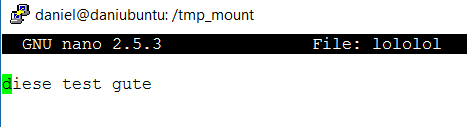
\includegraphics[width=0.5\linewidth]{images/edit.png}
		\caption{Editieren der gemeinsamen Datei}
		\label{edit}
	\end{center}
\end{figure}\

Versucht nun Client 1 ebenfalls die Datei zu editieren erhält man folgende Fehlermeldung:
\begin{figure}[!h]
	\begin{center}
		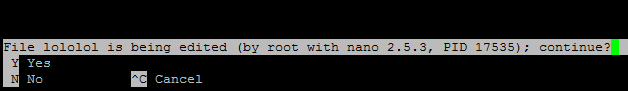
\includegraphics[width=0.8\linewidth]{images/error.png}
		\caption{Gleichzeitiges Editieren}
		\label{error}
	\end{center}
\end{figure}\

Im Endeffekt ist immer die letzte Aktion gültig und überschreibt die vorherigen Änderungen.
Dies ist jedoch nur möglich, da nano ein Journal führt und selbst die Datei lockt. Würde eine andere Applikation, welche diese Funktionalitäten nicht implementiert, eine Datei gleichzeitig von 2 verschiedenen Clients bearbeiten, würde diese korrupt werden. 